\section{Probing radiation}
This work is focussed on the use of X-ray and neutron scattering to probe soft matter systems; in particular surfactant monolayers and micelles. Therefore, it is pertinent to discuss how each of these probing radiation is produced and detail the advantages of each with respect to the other.

\subsection{Generation of X-rays}
X-rays are a form of electromagnetic radiation similar to visible light, albeit with a much shorter wavelength.\footnote{Typically \SIrange{0.01}{10}{\nano\meter}.}
There are four common ways to produce X-rays; three are available within the laboratory, while the other is exclusive to large scale facilities.

The three laboratory source X-ray generation techniques are the X-ray tube, the rotating anode, and the liquid jet.
An X-ray tube consists of a filament and an anode within a vacuum chamber, by passing a high voltage electrical current across the filament electrons are emitted which accelerate towards the anode.
On collision with the anode, the rapid deceleration results in the emission of X-rays at a characteristic wavelength based on the anode material.\autocite{schnablegger_saxs_2017}
The most common material for an X-ray tube anode is copper which gives off radiation with an energy of \SI{\sim8}{\kilo\eV}.\footnote{This is a wavelength of \SI{\sim1.5}{\nano\meter}.}

Another common laboratory method for the generation of X-rays is the rotating anode.\footnote{Essentially an improvement on the X-ray tube.}
In the X-ray tube, each time that an electron collides with anode there is some energy transfer, this means that over many millions of collisions the temperature of the anode can rise significantly, which can cause the anode material to melt.
Resulting in a temperature-based limitation to the available X-ray flux.
This lead to the development of the rotating anode, which is simply where the anode is made from a rotating wheel, such that the bombardment is spread across the whole wheel reducing the energy localisation.
The use of a rotating anode can allow for an increase in the photon flux by about an order of magnitude.\autocite{schnablegger_saxs_2017}

The final laboratory method for X-ray generation is the liquid jet source.\autocite[][Branded MetalJet by excillum]{noauthor_metaljet_nodate}
For the liquid jet X-ray source, an electron beam is incident on a liquid metal sample,\footnote{Usually an gallium or indium alloy.} rather than traditional solid metal, which can dissipate heat more efficiently.
This means that the electron intensity and therefore X-ray brightness, available to the liquid jet source is much greater than a rotating anode source.

The method of X-ray generation that is not available in a typical laboratory is at a synchrotron, the use of this method has the drawback that it requires access to a national or international facility.\footnote{Such as Diamond Light Source or the European Synchrotron Radiation Facility.}
The way in which X-rays are generated at a synchrotron involves the acceleration of an electron, rather than the deceleration as with the laboratory sources.
This is achieved by having relativistic electrons travel on a curve, from Newtonian mechanics it is known that travelling on a curve at constant speed is equivalent to acceleration.
First the electrons are accelerated, after being produced in a linear accelerator, to near the speed of light in a booster synchrotron before injecting them into the storage ring.
In the storage ring, the electrons are kept at relativistic speeds with bending magnets and straight sections making up a ring as shown in Figure~\ref{fig:syn}.
How circular the ring is depends on the number of bending magnets that make it up; for example, DLS had \num{48} bending magnets with \num{48} straight sections at the time of construction.
%
\begin{figure}[t]
    \centering
    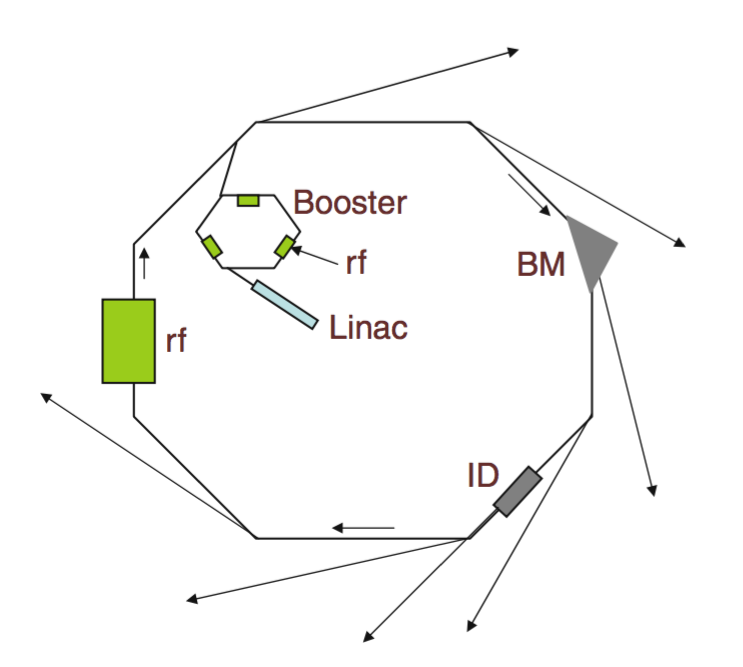
\includegraphics[width=0.7\textwidth]{theory/syn}
    \caption{A schematic representation of a synchrotron radiation source, identifying the Linac, the booster ring, the radio-frequency cavities (rf), the bending magnet (BM) and the insertion device (ID). Reprinted, with permission of Springer Nature Customer Service Centre GmbH: Springer Nature, from \cite{garcia-gutierrez_bases_2009}.}
    \label{fig:syn}
\end{figure}
%

When an electron accelerates (or travels on a curve), Cherenkov radiation is emitted in accordance with the Cherenkov relation,
%
\begin{equation}
    n_i\beta_c\cos{\theta_e} = 1,
\end{equation}
%
where, $n_i$ is the refractive index for the dielectric medium, $\beta_c$ is the fraction of the speed of light at which that electron is travelling, and $\theta_e$ is the angle between the electron trajectory and the trajectory of the resulting photon.\autocite{garcia-gutierrez_bases_2009}
The curve is the result of a bending magnet, meaning that at each bending magnet there can be a beamline which uses the synchrotron light.
The light that is given off from a bending magnet is continuous and broad, covering a wide range of the electromagnetic spectrum.
The alternative to a bending magnet beamline is that which is served by an insertion device.
An insertion device is able to offer more specific radiation characteristics (photon energy, narrower band) than a bending magnet, and are placed on the straight sections of the synchrotron.
Common insertion devices include wavelength shifters, wigglers, and undulators.

The type of insertion device that is present at both I07 and I22 at DLS is an undulator.
An undulator consists of a series of magnets of opposing polarity that causes the electrons to `wiggle' back and forth as shown in Figure~\ref{fig:undulator}.
This results in a superposition of radiation from $N_P$ sources, where $N_P$ is the number of magnets, yielding quasi-monochromatic radiation.
The brilliance of different X-ray sources are compared in Table \ref{tab:sources}, this shows the significant benefit that an undulator can offer in terms of photon brilliance.
%
\begin{marginfigure}
    \centering
    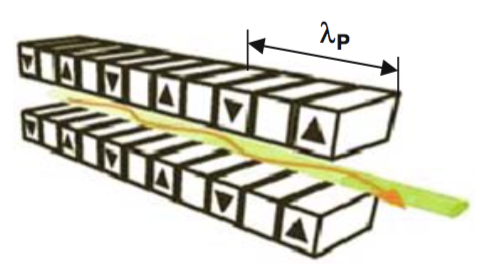
\includegraphics[width=\linewidth]{theory/undulator}
    \caption{A diagram of an undulator insertion device, such as that on I07 and I22, where $\lambda_P$ is the period length between opposing magnets. Reprinted, with permission of Springer Nature Customer Service Centre GmbH: Springer Nature, from \cite{garcia-gutierrez_bases_2009}.}
    \label{fig:undulator}
\end{marginfigure}
%
%
\begin{table}[t]
    \forceversofloat
    \centering
    \small
    \caption{A comparision of the photon brilliance from different light sources. Adapted, with permission of Oxford University Press, from \cite{sivia_elementary_2011}.}
    \label{tab:sources}
    \begin{tabular}{l | c}
        \toprule
        \multirow{2}{*}{Light source } & Approximate brilliance/ \\
 & \si{photons\,\second^{-1}\milli\radian^{-2}{0.1}\percent bandwidth^{-1}} \\
        \midrule
        Candle & \num{1e5} \\
        X-ray tube & \num{1e8} \\
        Sun & \num{1e10} \\
        Bending magnet & \num{1e15} \\
        Undulator & \num{1e20} \\
        \bottomrule
    \end{tabular}
\end{table}
%

\subsection{Generation of neutrons}
\label{sec:neutrons}
Neutrons hold an advantage over X-rays, particularly for application to the study of soft matter, due to the ability to use contrast variation to increase the quantity of information from the sample.\footnote{This is discussed in detail in Section~\ref{convar}.}
However, neutrons cannot be produced safely on a laboratory scale, therefore it is always necessary to visit large scale facilities to harness neutrons for scattering experiments.
These facilities come in two flavours; the reactor source and the spallation source, each offering unique benefits.

Neutron reactor sources\footnote{Such as the Institut Laue-Langevin (ILL) in Grenoble, France.} are currently the most common format of neutron source and are capable of producing the highest average neutron flux.\footnote{The number of neutrons per second per unit area.}
The High-Flux Reactor at the ILL is capable of producing a neutron flux of \SI{1.5E15}{neutrons\,\second^{-1}\centi\meter^{-2}}.\autocite{noauthor_ill_nodate}
A reactor source operates on the principle of nuclear fission, where an atomic nucleus is capable of breaking down into smaller nuclei, overcoming the strong nuclear force. This often involves using uranium enriched with its fissile isotope, \ce{^{235}U}, which after the initial absorption of a stray neutron\footnote{Arising from a cosmic ray, or spontaneous fission.} will undergo fission to release, on average, 2.5 daughter neutrons, an example of a possible uranium fission mechanism is:
%
\begin{equation*}
    \ce{n + ^{235}U -> ^{236}U -> ^{134}Xe + ^{100}Sr + 2n}.
\end{equation*}
%
This type of mechanism is the basis for both research, and nuclear power, reactors.\autocite{sivia_elementary_2011}
One of the major drawbacks for reactor neutron sources is the perceived public opinion towards such facilities.
Major safety concerns, such as ``nuclear meltdown'' and the resulting nuclear waste, mean that reactor sources are often unpopular and therefore struggle to obtain funding required for operation.

The other form of neutron source is a spallation source, this is much less controversial as it does not require fissile materials and hence there is no risk of a nuclear disaster.
The ISIS Neutron and Muon Source is an example of a spallation source, where high energy protons, \SI{800}{\mega\eV},\autocite{noauthor_isis_nodate-1} are accelerated towards a tungsten target.
When the protons strike the target, they can cause the release of a series of neutrons, the first batch of neutrons are given off with too high an energy to be useful, however, less excited neutrons are given off by secondary emissions.
In addition to the public perception benefit, spallation sources also offer a technological advantage in the time-of-flight\footnote{Abbreviated to ToF.} technique.
The ToF technique relies the fact that at a spallation source, it is possible to know the time at which the neutron was ejected from the target to a high level of precision and therefore it is possible to measure the time taken for the neutron to reach the instrument.
Since the neutron is a particle of a finite mass, $m$, it is possible to correlate the velocity, $\mathbf{v}$, of the particle with the kinetic energy, $E_k$,
%
\begin{equation}
    E_k = \frac{m\mathbf{v}^2}{2},
\end{equation}
%
and with knowledge of the energy of the particle, its wavelength, $\lambda$, can be determined by the de Broglie relation,\autocite{de_broglie_recherches_1925}
%
\begin{equation}
    E = h\omega = \frac{h\mathbf{v}}{\lambda},
\end{equation}
%
where, $h$ is Planck constant and $\omega$ is the neutron frequency.
Therefore, the wavelength of the neutron is proportional to the inverse of the particle's velocity, and hence the time-of-flight, $t_F$,
%
\begin{equation}
    \lambda = \frac{h}{m\mathbf{v}} = \frac{ht_F}{mL_F},
\end{equation}
%
where, $L_F$ is the distance between the target and the instrument.
The fact that the neutrons can spread out in the flight from the target means that wavelength-dispersive techniques, where the neutron wavelength is measured rather than the scattering angle, are possible at spallation sources which cannot be carried out natively at reactor sources.
The weakness of current spallation sources is that they have a lower average flux than reactor sources, however, the construction of the European Spallation Source will change this as it offers an average flux similar to that of a reactor source with the benefits of the spallation technique.

A problem that is inherent for both reactor and spallation sources is that the energy of the neutrons given off is usually too high to be used to study condensed materials, such as soft matter.
This means that moderation must be used to reduce the energy of the neutrons passing through the sample.
The neutrons that are considered to be optimal for the study of condensed materials are thermal in nature, named because their energy is approximately that of ambient temperature.
Thermal neutrons are achieved by allowing the neutrons to pass through a large volume of moderator material, usually, graphite, \ce{D2O}, methane or \ce{H2}, stored at \SI{300}{\kelvin} before they reach the instrument.\autocite{sivia_elementary_2011}

\subsection{Contrast variation}
\label{convar}
The scattering profile generated by the interaction of some system with radiation depends on three factors:
%
\begin{itemize}
    \item the spatial arrangement of the atoms in the system,
    \item the instrument being used to measure the pattern; instrumental resolution function, and
    \item the interaction between the radiation and the matter under investigation.
\end{itemize}
%
This final factor is perhaps better known as the ``scattering contrast'', this is an extremely important factor in the study of soft matter, particularly when the probing radiation is the neutron.
The scattering contrast makes it possible to select individual components of the system and investigate their structural properties.\autocite{schurtenberger_contrast_2002}
The differential cross-section, $\sfrac{\text{d}\sigma}{\text{d}\Omega}$ of a point scatterer, as shown in Equation~\ref{equ:sca}, varies only with respect to the scattering length of the species, $b$,
%
\begin{equation}
    \frac{\text{d}\sigma}{\text{d}\Omega} \propto b^2.
\end{equation}
%
However, as discussed in Section~\ref{sec:sld}, it is often easier to use the scattering length density.\footnote{Abbreviated to SLD.}.

When an X-ray interacts with an atom, it is scattered by the interaction with the electrons, this is due to the X-ray being a form of electromagnetic radiation.
Furthermore, it means that the scattering length of an atom by an X-ray is directly proportional to the number of electrons in the atom, so it is therefore it is difficult to discern between the scattering from a carbon atom (6 electrons) and a nitrogen atom,\footnote{As there is a difference of just a single electron between these atoms.}
Additionally, the scattering from hydrogen atoms is practically non-existent.

The scattering length a neutron by an atom varies unsystematically with respect to the atomic number of a species, this is shown in Figure~\ref{fig:scatlen}.
In addition to, the apparently random variation with changes in atomic number, there is also significant variation with mass number.\footnote{Leading to variation between isotopes of the same atom.}
This is also dependent on to the magnetic state of the atom, however, this is normally unimportant for soft matter.
The scattering lengths differ with the nuclear spin energy level, this leads to an average scattering length, $\langle b \rangle$, for isotopes where the nuclear spin is non-zero ($S\neq 0$).
There are two forms of scattering, coherent and incoherent, for which the scattering cross-sections, $\sigma$, are determined by,
%
\begin{equation}
    \begin{aligned}
        \sigma_{\text{coh}} & = 4\pi\langle b \rangle ^2 \\
        \sigma_{\text{incoh}} & = 4\pi(\langle b ^ 2 \rangle - \langle b \rangle ^2) \\
    \end{aligned}
\end{equation}
%
The coherent scattering is the scattering from nuclei that all have the same value of $\langle b \rangle$, and leads to the important scattering pattern.
Whereas, the incoherent scattering is caused by the `disorder' between the isotopes, and is the cause of the background present in the measurement.
Examples of these scattering cross-sections for nuclei relevant to soft matter are shown in Table~\ref{tab:crosssec}.
It can be seen that the incoherent scattering from the \ce{^1H} nuclei is more than forty times the coherent scattering.
This leads to a large, intrusive background present in the scattering pattern of hydrogenous samples.
%
\begin{figure}[t]
    \centering
    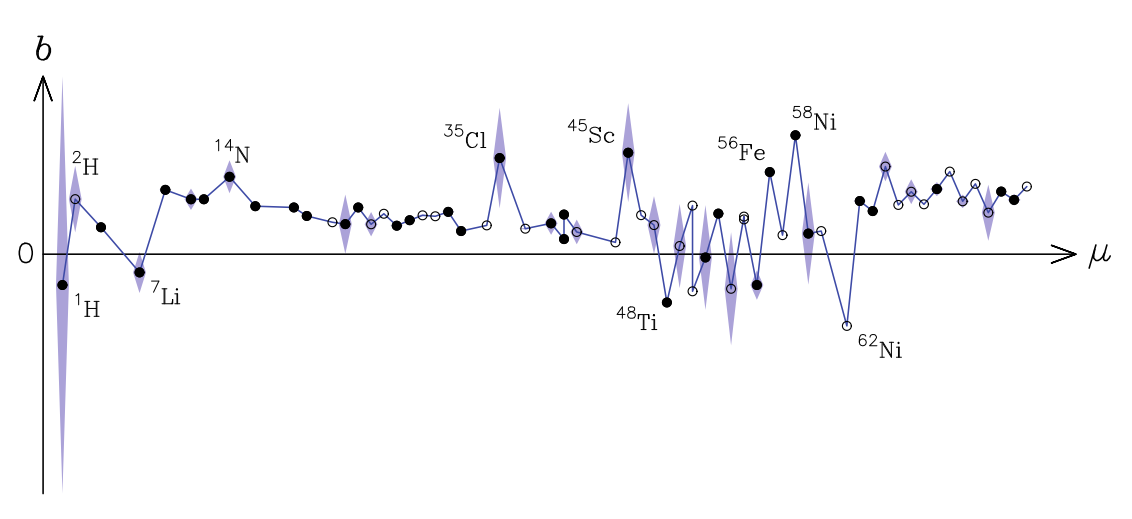
\includegraphics[width=0.85\textwidth]{theory/scatlen}
    \caption{The variation of the average neutron scatteirng length, $\langle b \rangle$ (circles), with atomic mass, $\mu$. The standard deviation, $\Delta b$, is indicated with the shaded regions. Reprinted, with permission of Oxford University Press, from \cite{sivia_elementary_2011}.}
    \label{fig:scatlen}
\end{figure}
%
\begin{table}[b]
    \centering
    \small
    \caption{Examples of coherent and incoherent scattering cross-sections. Reprinted, with permission of Elsevier, from \cite{schurtenberger_contrast_2002}.}
    \label{tab:crosssec}
    \begin{tabular}{r | c c c}
        \toprule
        Isotope & $S$ & $\sigma_{\text{coh}}$/\SI{e-28}{\meter\square} & $\sigma_{\text{incoh}}$/\SI{e-28}{\meter\square} \\
        \midrule
        \ce{^1H} & $\sfrac{1}{2}$ & 1.8 & 79.7 \\
        \ce{^2H} & 1 & 5.6 & 2.0 \\
        \ce{^{12}C} & 0 & 5.6 & -- \\
        \ce{^{14}N} & 1 & 11.6 & 0.3 \\
        \ce{^{16}O} & 0 & 4.2 & -- \\
        \bottomrule
    \end{tabular}
\end{table}
%
The difference between the scattering of \ce{^1H} and \ce{^2H}, evident in Table~\ref{tab:crosssec}, can lead to a very useful technique if soft matter scattering, known as contrast variation.
The idea of contrast variation is based on the substitution of one isotope of an atom for another, while not introducing significant change to the properties of the material.
Traditionally, the benefit of this came in terms of contrast matching out a part of the system to reduce the dimensionality of the problem for analysis.
For example, by matching the solvent SLD to that of the tails of the surfactants at the centre of a micelle there would only be scattered from the heads, and conversely, there would only be scattering from the tails if the solvent had the same SLD as the head groups.
This means that the problem becomes more straightforward as there are fewer variable parameters when fitting the data.
This idea is represented graphically in Figure~\ref{fig:convar}.
%
\begin{figure}[t]
    \forcerectofloat
    \centering
    
\includegraphics[width=\textwidth]{theory/convar}
    \caption{The effect of varying the SLD of the solvent in a micelle system, (a) the system in a pure solvent, (b) the solvent is contrast matched to the surfactant tails, and (c) the solvent is contrast matched to the surfactant heads.}
    \label{fig:convar}
\end{figure}
%
The technique of contrast variation may also be used in terms of data analysis.
By increasing the number of data sets corresponding to a single model at different contrasts, the solution for the true structure of the model from the scattering data becomes more robust.
This is due to the fact that each different contrast can be considered as an independent measurement of the same system, and hence each set of scattering data can be used within the data analysis procedure to obtain the best global agreement to the experiment.
This co-refinement of multiple experiments can, under the right conditions, be used to simultaneously consider both neutron and X-ray datasets.\autocite{nelson_co-refinement_2006}

 There is also the possibility of using contrast variation when the probing radiation is the X-ray, through the use of anomalous scattering.
This is where different wavelengths of radiation give different scattering when the wavelengths are on opposite sides of an X-ray absorption edge.
This is not frequently used for soft matter species, as the X-ray absorption edges for elements common in soft matter\footnote{H, C, N, O, etc.} are at very low X-ray energies so generally outside of the accessible range of a standard SAXS instrument.\autocite{schurtenberger_contrast_2002}
